 % % % % % % %% %PREAMBULO% % % % % % % % % % %
\documentclass[a4paper,12pt]{report}

\usepackage{fancyhdr}
\usepackage[utf8]{inputenc}
\usepackage{minted}
\usepackage{graphicx}
\usepackage[portuguese]{babel}
\usepackage{mdframed}

\usepackage{geometry}
 \geometry{
 a4paper,
 total={170mm,257mm},
 left=20mm,
 top=20mm,
 }
 
\usemintedstyle{bw}

\pagestyle{fancy}\lhead{ Análise Léxica e Sintática LALR } \rhead{DCC053 - Trabalho Prático 1}
\renewcommand{\contentsname}{Índice}
\renewcommand\thesection{\arabic{section}}

 % % % % % % %% %DOCUMENTO% % % % % % % % % % %

\begin{document}

% Capa
\begin{titlepage}
	\centering
	{\scshape\LARGE Universidade Federal de Minas Gerais \par}
	{\scshape\Large Instituto de Ciências Exatas \par}
	{\scshape\Large Departamento de Ciência da Computação \par}
	\vfill
	{\huge\bfseries \textbf{Compiladores I - DCC053} \par}
	{\huge\bfseries \textbf{Trabalho Prático 1\\Análise Léxica e Sintática LALR} \par}
	\vfill
	{\Large Hugo Araújo de Sousa\\(2013007463)\par}
	\vfill
	{\large 2º Semestre de 2017\par}
\end{titlepage}

\newpage

\section{Descrição do Problema}

Em projetos de compiladores modernos, as etapas iniciais do processo de análise
do código fonte são as análises Léxica e Sintática. Durante a análise léxica, o
programa fonte é organizado em tokens, que são sequências significativas para
a linguagem em questão. Com esses tokens, pode-se contruir a tabela de símbolos,
necessária para a fase posterior de análise semântica e de geração de código.

Já a fase de análise sintática é responsável por, a partir dos tokens produzidos
inicialmente, impor uma estrutura gramatical sobre o programa fonte.

Nesse trabalho, são implementadas as fases de análise léxica e sintática para
a linguagem de programação definida através da gramática mostrada na Figura
\ref{fig:gramatica}.

\begin{figure}[h]
 \centering
 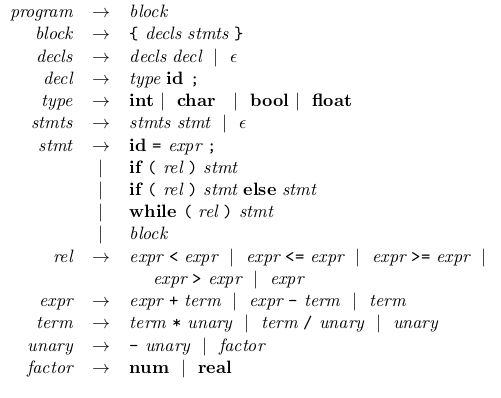
\includegraphics[scale=0.7]{grammar.png}
 \caption{Gramática da linguagem para qual a análise léxica e sintática será feita.}
 \label{fig:gramatica}
\end{figure}

\section{Metodologia}

O trabalho foi realizado utilizando a linguagem de programação Java. Para esta,
existem ferramentas que auxiliam no desenvolvimento de analisadores léxico e
sintáticos. Nesse trabalho foram utilizadas as ferramentas JLex e Cup, que
funcionam de forma coordenada.

Para gerar analisadores léxicos, a ferramenta JLex se mostra de grande utilidade,
uma vez que permite que os tokens da linguagem sejam especificados através das 
expressões regulares correspondentes. Dessa forma, o problema de gerar um
analisador léxico é reduzido ao problema de determinar expressões regulares
para cada um dos tokens da linguagem.

Já para gerar analisadores sintáticos, a ferramenta CUP funciona de forma coordenada
com o JLex. Nela, basta escrever, usando a sintaxe apropriada, as regras da gramática
da linguagem. Além disso também pode-se especificar outras ações do analisador de acordo
com as necessidades do usuário.

\section{Compilação e Uso}

Para facilitar a compilação do projeto, foi disponibilizado um arquivo Makefile.
Nele, há cinco alvos: \textbf{clean}, limpa a compilação do projeto; \textbf{lex},
compila o analisador léxico; \textbf{cup}, compila o analisador sintático;
\textbf{all}, compila ambos os analisadores e \textbf{run} executa os analisadores.

Além disso, para configurar corretamente o projeto, é necessário incluir os arquivos
necessários às ferramentas JLex e CUP, como mostrado na Figura \ref{fig:folder}.

\begin{figure}[h]
 \centering
 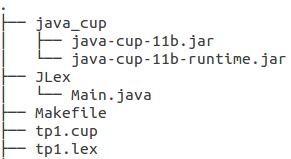
\includegraphics[scale=0.7]{folder.png}
 \caption{Estrutura do diretório do projeto.}
 \label{fig:folder}
\end{figure}

Ao executar os analisadores, o programa fonte passado como entrada é analisado
léxica e sintaticamente. Na saída, o programa fonte é impresso até onde o analisador
léxico é bem sucedido, dessa forma, ao ocorrer um error léxico, o mesmo é registrado
no ponto do programa onde ocorreu.

Caso a análise léxica seja completada sem erros, o analisador sintático imprimirá,
em caso de sucesso, todas as produções gramaticais utilizadas no programa e uma mensagem
indicando sucesso.

Além disso, em caso de sucesso, todos os tokens presentes no programa fonte serão impressos
em um arquivo de texto no diretório do projeto.

\section{Testes e Resultados}

A fim de ilustar o uso dos analisadores desenvolvidos, nessa seção são mostrados
dois exemplos de teste.

\subsection{input1.txt}

\begin{itemize}
 \item Entrada
 
 \begin{mdframed}[linecolor=black, leftline=false, rightline=false, backgroundcolor=gray!20!white]
    \inputminted[linenos, fontsize=\footnotesize]{text}{../src/input/input1.txt}
\end{mdframed}
 
 \item Saída

\begin{mdframed}[linecolor=black, leftline=false, rightline=false, backgroundcolor=gray!20!white]
    \inputminted[linenos, fontsize=\footnotesize]{text}{../src/tokens1.txt}
\end{mdframed}
 
\begin{mdframed}[linecolor=black, leftline=false, rightline=false, backgroundcolor=gray!20!white]
    \inputminted[linenos, fontsize=\footnotesize]{text}{../src/output1.txt}
\end{mdframed}
 
\end{itemize}

\subsection{input2.txt}

\begin{itemize}
 \item Entrada
 
 \begin{mdframed}[linecolor=black, leftline=false, rightline=false, backgroundcolor=gray!20!white]
    \inputminted[linenos, fontsize=\footnotesize]{text}{../src/input/input2.txt}
\end{mdframed}
 
 \item Saída
 
\begin{mdframed}[linecolor=black, leftline=false, rightline=false, backgroundcolor=gray!20!white]
    \inputminted[linenos, fontsize=\footnotesize]{text}{../src/tokens2.txt}
\end{mdframed}

\begin{mdframed}[linecolor=black, leftline=false, rightline=false, backgroundcolor=gray!20!white]
    \inputminted[linenos, fontsize=\footnotesize]{text}{../src/output2.txt}
\end{mdframed}
 
\end{itemize}

\section{Código Fonte}

\subsection{tp1.lex}

\begin{mdframed}[linecolor=black, leftline=false, rightline=false, backgroundcolor=gray!20!white]
    \inputminted[linenos, fontsize=\footnotesize]{text}{../src/tp1.lex}
\end{mdframed}

\subsection{tp1.cup}

\begin{mdframed}[linecolor=black, leftline=false, rightline=false, backgroundcolor=gray!20!white]
    \inputminted[linenos, fontsize=\footnotesize]{text}{../src/tp1.cup}
\end{mdframed}

\subsection{Makefile}

\begin{mdframed}[linecolor=black, leftline=false, rightline=false, backgroundcolor=gray!20!white]
    \inputminted[linenos, fontsize=\footnotesize]{text}{../src/Makefile}
\end{mdframed}

\section{Referências}

\begin{itemize}
 \item Aho, A.V.; Sethi, R.; Ullman, J.D. Compilers Principles, Techniques, and
 Tools, Addison Wesley, 1986.
\end{itemize}


\end{document}